\section{Netzplan}
Im folgenden Netzplan (Abbildung~\ref{fig:netzplan}) sind alle Arbeitspakete der Entwicklung des Avocado-Share dargestellt. 
Um sicherzustellen, dass jedes Arbeitspaket termingerecht und vollständig ausgeführt wird, haben wir beschlossen, neben dem Verantwortlichen auch eine Person zu bestimmen, welche eine Aufgabe ausführt.\\

Durch eine Planungsphase zu Beginn des Projektes, ist es uns möglich eine klare Schichtentrennung zu machen.
Da wir in der Planung die Schnittstellen zwischen den Schichten definieren, ist es uns möglich die Entwicklungsschritte danach
alle parallel auszuführen. Dadurch erhalten wir zwar einen kleinen Flaschenhals beim Erstellen der Grobstruktur und des
Grundgerüstes, doch es bringt uns viel Freiheit in den folgenden Paketen. So können wir besser und einfacher auf allfällige
Verzögerungen und Ausfälle reagieren.
Da wir eine technisch saubere Lösung haben wollen, ist es uns wichtig, dass die Spezialisten eines Bereiches in unserem Team auch entweder Verantwortlicher oder Ausführender eines Arbeitspaketes sind. \\

Ein Paket gilt erst als abgeschlossen, wenn die Qualität der Arbeit überprüft wurde.
Für geschriebenen Java-Code, sollen Unit-Tests geschrieben werden. Bei Web- und UI-Paketen sollte ein kurzes Test-Protokoll geschrieben werden, um sicherzustellen, dass alle Module und Klassen auch korrekt implementiert wurden und funktionieren.
So kann beim Arbeitspaket "`Testing"' schnell und einfach alles nochmals getestet werden. Design- und Planungspakete, wie "`Softwareentwurf"' oder "`DB-Deisgn"', müssen zur Kontrolle einem Review des Projektteams standhalten.\\

Im Anhang~\ref{sub:arbeitspakete_und_aufwandschaetzung} finded sich eine Auflistung aller Arbeitspakete. Ebenfalls ist unter \ref{sec:netzplan_abhaengigkeiten} eine zusätzliche Darstellung des Netzplanes zu finden, bei welcher die Pakete nach ihren Abhängigkeiten gegliedert sind. Diese zustätzliche Darstellung zeigt, welche Schritte parallel erledigt werden könnten.

\begin{landscape}
% \vspace*{\fill}: center vertically 
% source: https://stackoverflow.com/questions/3141702/vertically-centering-a-title-page
\vspace*{\fill}
\begin{figure}[H]
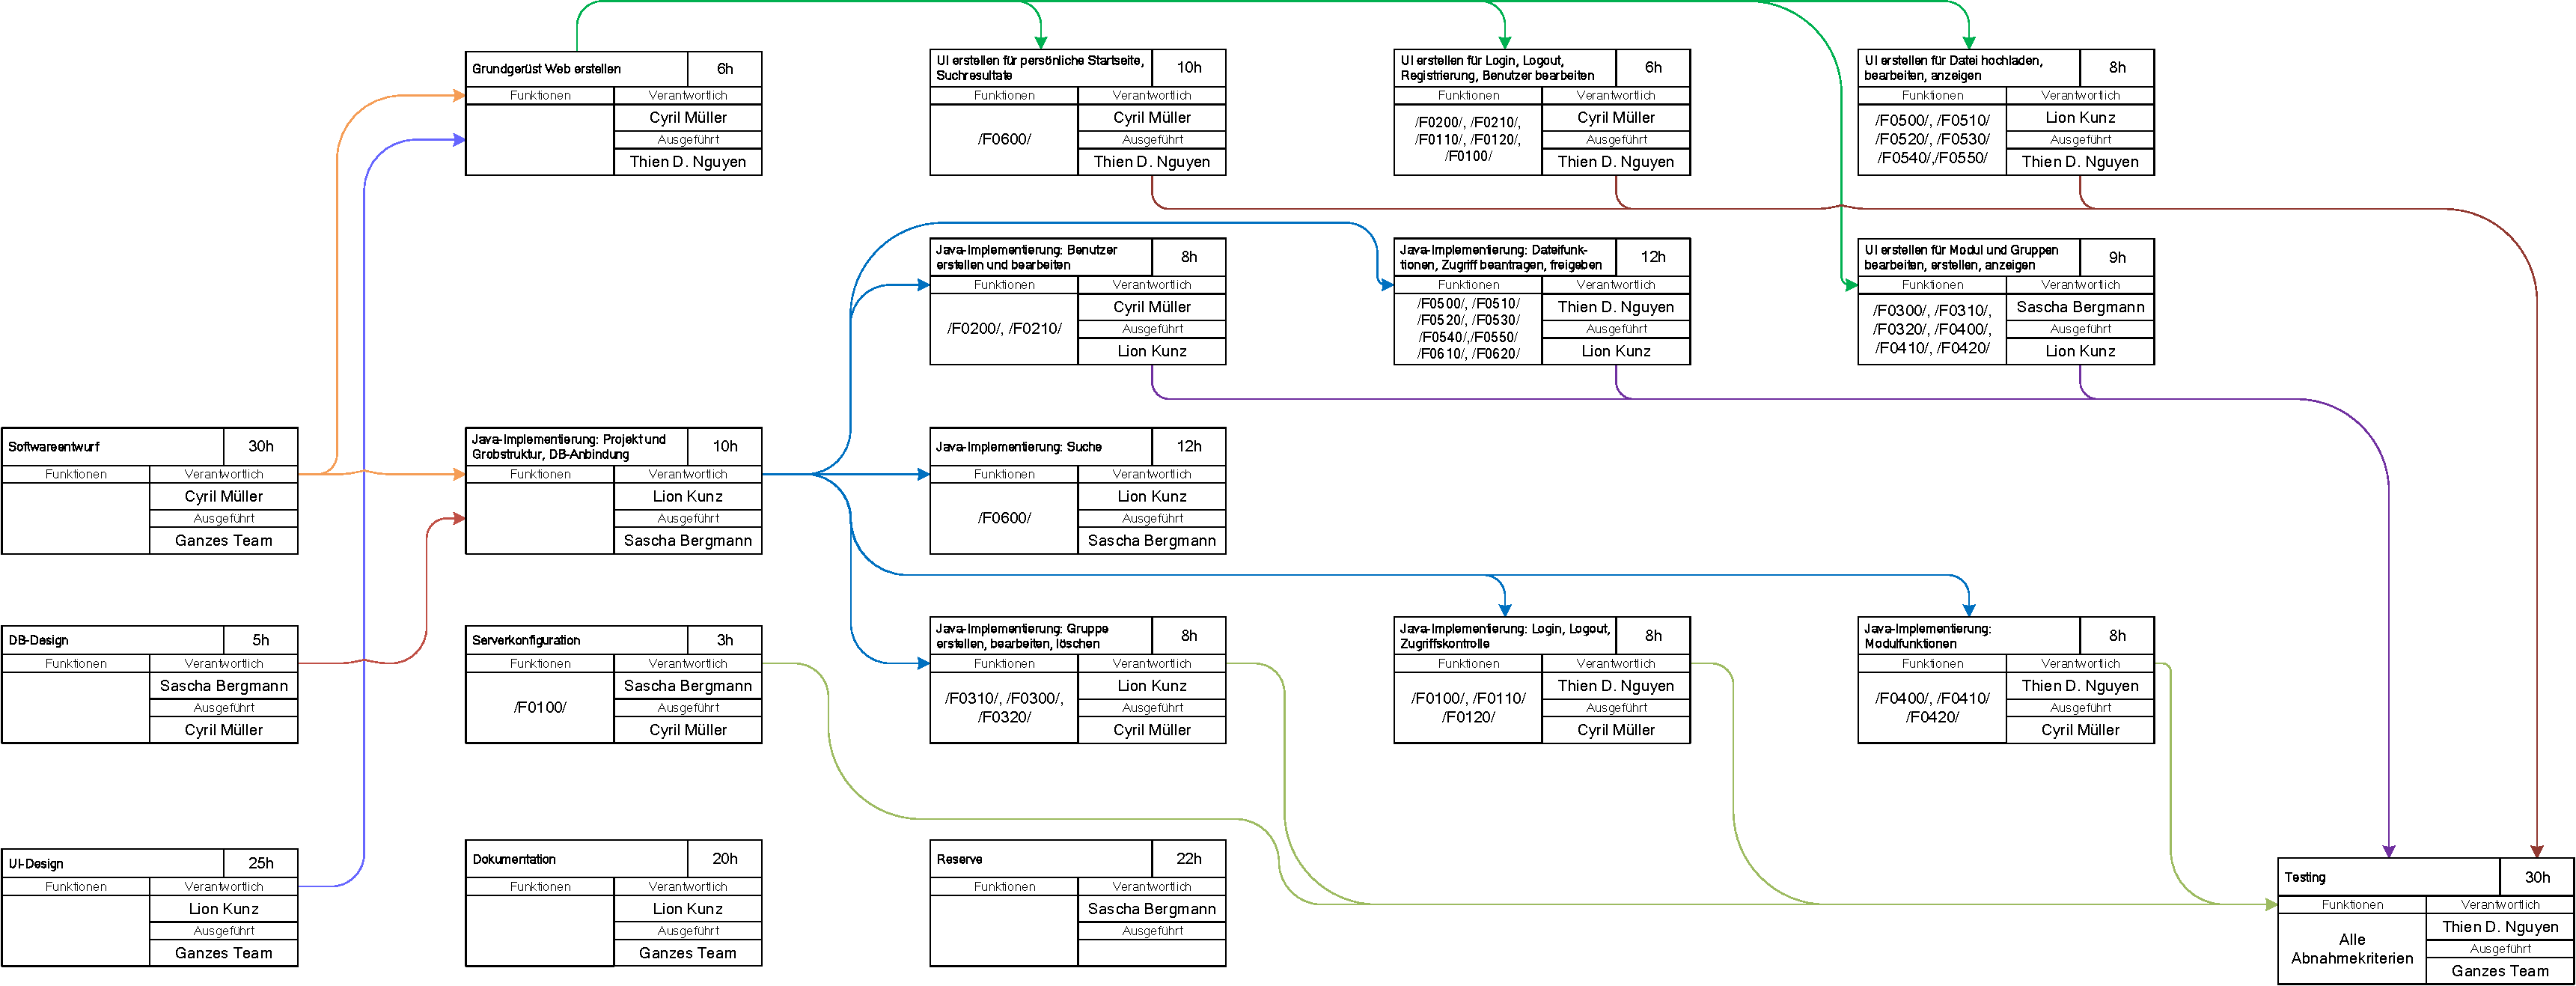
\includegraphics[width=\linewidth]{graphics/netzplan_s2.pdf}
\caption{Der Netzplan zeigt die Arbeitspakete, geordnet nach Arbeitsprozessen.}
\label{fig:netzplan}
\end{figure}
\vspace*{\fill}
\end{landscape}
